\documentclass{article}

\usepackage[spanish]{babel}
\usepackage[utf8]{inputenc}
\usepackage[T1]{fontenc}
\usepackage{graphicx}
\usepackage{hyperref}
\usepackage{courier}
\usepackage{listings}
\usepackage{xcolor}
\usepackage{blindtext}
\usepackage{scrextend}
\usepackage[document]{ragged2e}
\usepackage{multicol}
\usepackage{pgfgantt}
\usepackage{minted}
\usepackage{tikz}
\usepackage{longtable}
\usepackage{algorithm}
\usepackage[noend]{algpseudocode}
\usepackage{amsmath}
\usepackage{wrapfig,lipsum,booktabs}
\usepackage{fontspec}
 % % % % % % % %

\setmainfont{Calibri}

\hypersetup{
	colorlinks,
	linkcolor={blue!60!black},
	citecolor={blue!50!black},
	urlcolor={blue!80!black}
}

\usetikzlibrary{positioning,fit,calc}

\usemintedstyle{pastie}

\usepackage{array}
\newcolumntype{L}[1]{>{\raggedright\let\newline\\\arraybackslash\hspace{0pt}}m{#1}}
\newcolumntype{C}[1]{>{\centering\let\newline\\\arraybackslash\hspace{0pt}}m{#1}}
\newcolumntype{R}[1]{>{\raggedleft\let\newline\\\arraybackslash\hspace{0pt}}m{#1}}

\def\labelitemi{\textbf{--}}

\usepackage{anysize}
\marginsize{2.54cm}{2.54cm}{2.54cm}{2.54cm}

\usepackage{setspace}
%\onehalfspacing
\doublespacing

\makeatletter
\newcommand*{\MoveFitHeight}[1]{%
	\pgfmathsetlengthmacro\fit@inner@sep{%
		\pgfkeysvalueof{/pgf/inner xsep}%
	}%
	\pgfmathsetlengthmacro\fit@text@height{%
		\tikz@text@height
	}%
	\kern-\fit@inner@sep\relax
	\raisebox{\fit@text@height}[0pt][0pt]{#1}%
}
\makeatother

\newcommand{\bigO}[1]{$O({#1})$}

\setlength{\columnsep}{1cm}

%En caso de que LaTeX separe las palabras con - de manera incorrecta, usar
%\hyphenation{deci-sión,e-xa-men, otras palabras....}

% %PORTADA
\begin{document}
\title{Algoritmos de Planificación del Procesador}
\author{Victor Tortolero}

\centerline{Universidad de Carabobo}
\centerline{Facultad de Ciencia y Tecnologia}
\centerline{Sistemas Operativos}

\vspace{8cm}
\begin{centering}
\hrule 	\vspace{0.4cm}
	{ \Huge \bfseries Algoritmos de Planificación del Procesador \\[0.4cm] }
\hrule \vfill
\end{centering}

\vfill
\centerline{Victor Tortolero, 24.569.609}


\centerline{\today}

\newpage
% %Fin Portada


\flushleft
\setlength{\parindent}{20pt}


%%CUERPO PRINCIPAl%%%%%%%%%%%%%%%%%%%%%%%%%%%%%%%%%%%%%%%%%%%	
\justify

% First Come First Serve (FCFS) %---------------------------------------------
{\centering \section{First Come First Serve (FCFS)}}

Con este algoritmo los procesos se van ingresando en una cola FIFO(First In, First Out), 
al llegar el proceso se inserta su PCB en la cola, luego si el CPU esta libre toma el primer
elemento de la cola y se elimina este de la cola. Como es no apropiativo, la CPU solo toma
otro proceso de la cola al terminar el actual. Para implantar este algoritmo solo se requiere una cola FIFO.

\begin{itemize}
	\item \textbf{Ventajas}
	\begin{itemize}
			\item Es fácil de entender e implementar.
	\end{itemize}

	\item \textbf{Desventajas}
	\begin{itemize}
		\item Aunque normalmente es justo en como dedica tiempo de CPU a los procesos,
		los procesos largos hacen esperar a los cortos.
		\item El tiempo de espera es alto por lo que carece de rendimiento.
	\end{itemize}
\end{itemize}

Supongamos que tenemos 3 procesos:
\begin{center}
	\begin{tabular}{|c|c|} \hline
		Proceso & Tiempo de Ráfaga \\ \hline
		$P_{0}$ & 20 \\
		$P_{1}$ & 6 \\
		$P_{2}$ & 9 \\ \hline
	\end{tabular}
\end{center}

\vspace{0.4cm}

Si los procesos llegan en el siguiente orden, $P_{0} \rightarrow P_{1} \rightarrow P_{2}$, tendríamos el diagrama de gantt \ref{gantt:FCFS1},
y el tiempo de espera promedio seria $\frac{0 + 20 + 26}{3} = 15.333ms$. \newline
En cambio si los procesos llegaran en el orden $P_{1} \rightarrow P_{2} \rightarrow P_{0}$, tendríamos el diagrama de gantt \ref{gantt:FCFS2},
y el tiempo de espera promedio seria $\frac{0 + 6 + 15}{3} = 8ms$. \newline
En este algoritmo es importante el orden en el que llegan los procesos, y si el tiempo entre ellos varia de gran manera, entonces tendremos
un tiempo de espera alto.

\vspace{0.4cm}

\begin{figure}[h]
	\centering
	\begin{minipage}{0.45\textwidth}
		\centering
		\caption{FCFS, Ejemplo 1}
		\begin{tikzpicture}[box/.style={draw,minimum width=2cm, minimum height=1cm,align=center}, node distance=0cm and 0cm]
		\node[box, minimum width=4cm] (N1) {$P_{0}$};
		\node[box, minimum width=0.6cm, right=of N1] (N2) {$P_{1}$};
		\node[box, minimum width=1cm, right=of N2] (N3) {$P_{2}$};
		\node[yshift=-1.5cm, inner sep=2pt, fit={(N1) (N2)}, align=left] (fit) {\MoveFitHeight{0}};
		\node[yshift=-1.5cm, inner sep=2pt, fit={(N2) (N3)}, align=left,] (fit) {\MoveFitHeight{20}};
		\node[yshift=-1.5cm, inner sep=2pt, fit={(N3) (N3)}, align=left,] (fit) {\MoveFitHeight{26}};
		\node[yshift=-1.5cm, inner sep=2pt, fit={(N3) (N3)}, align=right,] (fit) {\MoveFitHeight{35}};
		\end{tikzpicture}
		\label{gantt:FCFS1}
	\end{minipage}\hfill
	\begin{minipage}{0.45\textwidth}
		\centering
		\caption{FCFS, Ejemplo 2}
		\begin{tikzpicture}[box/.style={draw,minimum width=2cm, minimum height=1cm,align=center}, node distance=0cm and 0cm]
		\node[box, minimum width=0.6cm] (N1) {$P_{1}$};
		\node[box, minimum width=1cm, right=of N1] (N2) {$P_{2}$};
		\node[box, minimum width=4cm, right=of N2] (N3) {$P_{0}$};
		\node[yshift=-1.5cm, inner sep=2pt, fit={(N1) (N2)}, align=left,] (fit) {\MoveFitHeight{0}};
		\node[yshift=-1.5cm, inner sep=2pt, fit={(N2) (N3)}, align=left,] (fit) {\MoveFitHeight{6}};
		\node[yshift=-1.5cm, inner sep=2pt, fit={(N3) (N3)}, align=left,] (fit) {\MoveFitHeight{15}};
		\node[yshift=-1.5cm, inner sep=2pt, fit={(N3) (N3)}, align=right,] (fit) {\MoveFitHeight{35}};
		\end{tikzpicture}
		\label{gantt:FCFS2}
	\end{minipage}
\end{figure}
\newpage
%----------------------------------------------------------------------------------%


% Shortest Job First (SJF) %---------------------------------------------
{\centering \section{Shortest Job First (SJF)}}

Este algoritmo selecciona el proceso con el próximo tiempo de ejecución mas corto(El que tenga
la próxima ráfaga de CPU mas corta).
Asocia con cada proceso la duración de la siguiente ráfaga de CPU del proceso.
Cuando el CPU esta libre se le asigna el proceso que tiene la siguiente ráfaga de CPU
mas corta. Si varios procesos tienen la misma duración de ráfaga, se usa el algoritmo
FCFS para elegir el proceso. 

Para implantar este algoritmo se requiere una cola, y una método para saber la duración de la siguiente ráfaga
de CPU para los procesos en la cola, normalmente se usan métodos para hacer aproximaciones o predecir la siguiente rafaga
mediante las ráfagas
ya conocidas.
Este algoritmo pudiera ser el mas rápido, pero es difícil conocer la duración de la siguiente ráfaga.
\begin{itemize}
	\item \textbf{Ventajas}
	\begin{itemize}
		\item Tiempo promedio de espera reducido.
	\end{itemize}
	
	\item \textbf{Desventajas}
	\begin{itemize}
		\item Difícil de implementar ya que es complicado conocer la duración de la siguiente ráfaga
		de CPU para un proceso.
	\end{itemize}
\end{itemize}

Supongamos que tenemos 4 procesos y que todos llegan al mismo tiempo:
\begin{center}
	\begin{tabular}{|c|c|c|} \hline
		Proceso & Tiempo de Ráfaga(ms) & Tiempo de llegada(ms) \\ \hline
		$P_{0}$ & 6 & 0 \\
		$P_{1}$ & 8 & 0 \\
		$P_{2}$ & 7 & 0 \\
		$P_{3}$ & 3 & 0 \\ \hline
	\end{tabular}
\end{center}

\vspace{0.4cm}

En este caso tenemos un tiempo promedio de espera $\frac{0 + 3 + 9 + 16}{4} = 7ms$.

\vspace{0.4cm}

\begin{figure}[h]
	\centering
	\begin{minipage}{0.45\textwidth}
		\centering
		\caption{SJF, Ejemplo}
		\begin{tikzpicture}[box/.style={draw,minimum width=2cm, minimum height=1cm,align=center}, node distance=0cm and 0cm]
			\node[box, minimum width=1cm] (N1) {$P_{3}$};
			\node[box, minimum width=1cm, right=of N1] (N2) {$P_{0}$};
			\node[box, minimum width=1.8cm, right=of N2] (N3) {$P_{2}$};
			\node[box, minimum width=1.5cm, right=of N3] (N4) {$P_{1}$};
			\node[, yshift=-1.5cm, inner sep=2pt, fit={(N1) (N2)}, align=left,] (fit) {\MoveFitHeight{0}};
			\node[, yshift=-1.5cm, inner sep=2pt, fit={(N2) (N3)}, align=left,] (fit) {\MoveFitHeight{3}};
			\node[, yshift=-1.5cm, inner sep=2pt, fit={(N3) (N4)}, align=left,] (fit) {\MoveFitHeight{9}};
			\node[, yshift=-1.5cm, inner sep=2pt, fit={(N4) (N4)}, align=left,] (fit) {\MoveFitHeight{16}};
			\node[, yshift=-1.5cm, inner sep=2pt, fit={(N4) (N4)}, align=right,] (fit) {\MoveFitHeight{24}};
		\end{tikzpicture}
		\label{gantt:SJF1}
	\end{minipage}\hfill
\end{figure}
\newpage
%----------------------------------------------------------------------------------%


% Shortest Remaining Time First (SRTF) %----------------------------------------------%
{\centering \section{Shortest Remaining Time First (SRTF)}}

Este algoritmo selecciona el proceso que esta en ejecución con otro que exija menor tiempo total de ejecución.
Consigue una buena eficiencia, ya que logra que la lista de procesos preparados sea lo más corta posible. 

Para implantar este algoritmo necesitamos una cola, y conocer el tiempo total de cada proceso.

\begin{itemize}
	\item \textbf{Ventajas}
	\begin{itemize}
		\item Es eficiente.
		\item Presenta un buen tiempo promedio de servicio.
		\item Logra que la lista de procesos preparados sea lo más corta posible. 
	\end{itemize}
	
	\item \textbf{Desventajas}
	\begin{itemize}
		\item Los procesos largos no se ejecutaran mientras existan procesos cortos 
		en la cola.
	\end{itemize}
\end{itemize}

Supongamos que tenemos 4 procesos:
\begin{center}
	\begin{tabular}{|c|c|c|} \hline
		Proceso & Tiempo de Ráfaga(ms) & Tiempo de llegada(ms) \\ \hline
		$P_{0}$ & 20 & 3 \\
		$P_{1}$ & 6 & 2 \\
		$P_{2}$ & 24 & 0 \\
		$P_{3}$ & 8 & 1 \\ \hline
	\end{tabular}
\end{center}

Primero el CPU trataría el $P_{2}$ ya que es el primero en entrar a la cola,
luego cuando llega el $P_{3}$ el algoritmo verifica y tenemos que el tiempo que le queda
a $P_{2}$(23ms) es mayor al tiempo que le queda a $P_{3}$(8ms), por lo que el CPU trata a $P_{3}$.
Siguiendo estas reglas tendríamos el diagrama de gantt \ref{gantt:SJF1}.

\vspace{0.4cm}

\begin{figure}[h]
	\centering
	\begin{minipage}{1\textwidth}
		\centering
		\caption{Tiempo de espera Promedio: $\frac{0 + 1 + 2 + 8 + 15 + 35}{6} = 10.166ms$}
		\begin{tikzpicture}[box/.style={draw,minimum width=2cm, minimum height=1cm,align=center}, node distance=0cm and 0cm]
		\node[box, minimum width=0.6cm] (N1) {$P_{0}$};
		\node[box, minimum width=1cm, right=of N1] (N2) {$P_{1}$};
		\node[box, minimum width=1.3cm, right=of N2] (N3) {$P_{3}$};
		\node[box, minimum width=1.7cm, right=of N3] (N4) {$P_{0}$};
		\node[box, minimum width=2.2cm, right=of N4] (N5) {$P_{2}$};
		\node[yshift=-1.5cm, inner sep=2pt, fit={(N1) (N2)}, align=left,] (fit) {\MoveFitHeight{0}};
		\node[yshift=-1.5cm, inner sep=2pt, fit={(N2) (N3)}, align=left,] (fit) {\MoveFitHeight{1}};
		\node[yshift=-1.5cm, inner sep=2pt, fit={(N3) (N4)}, align=left,] (fit) {\MoveFitHeight{5}};
		\node[yshift=-1.5cm, inner sep=2pt, fit={(N4) (N5)}, align=left,] (fit) {\MoveFitHeight{11}};
		\node[yshift=-1.5cm, inner sep=2pt, fit={(N5) (N5)}, align=left,] (fit) {\MoveFitHeight{20}};
		\node[yshift=-1.5cm, inner sep=2pt, fit={(N5) (N5)}, align=right,] (fit) {\MoveFitHeight{32}};
		\end{tikzpicture}
		\label{gantt:SJF1}
	\end{minipage}\hfill
\end{figure}
\newpage
%----------------------------------------------------------------------------------%


% Round Robin (RR) %---------------------------------------------------------------%
{\centering \section{Round Robin (RR)}}

Consiste en conceder a cada proceso en ejecución un determinado período de tiempo, denominado quantum (Q), transcurrido el cual,
si el proceso no ha terminado, se le devuelve al final de la cola de procesos preparados y se pasa al proceso
que este de primero en la cola.
Esta interrupción periódica continúa hasta que el proceso termine su ejecución, formando una rueda de procesos que 
serán ejecutados cíclicamente hasta que terminen.

Para su implantación requiere una cola (circular) y el valor optimo de Q, el cual se determina según
el tipo de sistema y el numero de procesos.

\begin{itemize}
	\item \textbf{Ventajas}
	\begin{itemize}
		\item Es justo con todos los procesos.
	\end{itemize}
	
	\item \textbf{Desventajas}
	\begin{itemize}
		\item Si el valor de Q es mayor que el tiempo requerido 
		por el proceso mas largo, se convierte en FCFS.
		\item Si el valor de Q es muy pequeño se producen muchos
		cambios de contexto lo que es ineficiente.
	\end{itemize}
\end{itemize}

Supongamos que tenemos 3 procesos:
\begin{center}
	\begin{tabular}{|c|c|c|} \hline
		Proceso & Tiempo de Ráfaga(ms) & Tiempo de llegada(ms) \\ \hline
		$P_{0}$ & 5 & 0 \\
		$P_{1}$ & 3 & 1 \\
		$P_{2}$ & 8 & 2 \\ \hline
	\end{tabular}
\end{center}

Para Q = 4,  y Q = 8 tenemos:

\vspace{0.4cm}

\begin{figure}[h]
	\centering
	\begin{minipage}{0.45\textwidth}
		\centering
		\caption{Q = 4}
		\begin{tikzpicture}[box/.style={draw,minimum width=2cm, minimum height=1cm,align=center}, node distance=0cm and 0cm]
		\node[box, minimum width=1.2cm] (N1) {$P_{0}$};
		\node[box, minimum width=0.9cm, right=of N1] (N2) {$P_{1}$};
		\node[box, minimum width=1.2cm, right=of N2] (N3) {$P_{2}$};
		\node[box, minimum width=0.6cm, right=of N3] (N4) {$P_{0}$};
		\node[box, minimum width=1.2cm, right=of N4] (N5) {$P_{2}$};
		\node[yshift=-1.5cm, inner sep=2pt, fit={(N1) (N2)}, align=left,] (fit) {\MoveFitHeight{0}};
		\node[yshift=-1.5cm, inner sep=2pt, fit={(N2) (N3)}, align=left,] (fit) {\MoveFitHeight{4}};
		\node[yshift=-1.5cm, inner sep=2pt, fit={(N3) (N4)}, align=left,] (fit) {\MoveFitHeight{7}};
		\node[yshift=-1.5cm, inner sep=2pt, fit={(N4) (N5)}, align=left,] (fit) {\MoveFitHeight{11}};
		\node[yshift=-1.5cm, inner sep=2pt, fit={(N5) (N5)}, align=left,] (fit) {\MoveFitHeight{12}};
		\node[yshift=-1.5cm, inner sep=2pt, fit={(N5) (N5)}, align=right,] (fit) {\MoveFitHeight{16}};
		\end{tikzpicture}
		\label{gantt:RR1}
	\end{minipage}\hfill
	\begin{minipage}{0.45\textwidth}
		\centering
		\caption{Q = 8}
		\begin{tikzpicture}[box/.style={draw,minimum width=2cm, minimum height=1cm,align=center}, node distance=0cm and 0cm]
		\node[box, minimum width=1.2cm] (N1) {$P_{0}$};
		\node[box, minimum width=0.9cm, right=of N1] (N2) {$P_{1}$};
		\node[box, minimum width=1.6cm, right=of N2] (N3) {$P_{2}$};
		\node[yshift=-1.5cm, inner sep=2pt, fit={(N1) (N2)}, align=left,] (fit) {\MoveFitHeight{0}};
		\node[yshift=-1.5cm, inner sep=2pt, fit={(N2) (N3)}, align=left,] (fit) {\MoveFitHeight{5}};
		\node[yshift=-1.5cm, inner sep=2pt, fit={(N3) (N3)}, align=left,] (fit) {\MoveFitHeight{8}};
		\node[yshift=-1.5cm, inner sep=2pt, fit={(N3) (N3)}, align=right,] (fit) {\MoveFitHeight{16}};
		\end{tikzpicture}
		\label{gantt:RR2}
	\end{minipage}
\end{figure}
\newpage
%----------------------------------------------------------------------------------%


%--% Prioridades %-----------------------------------------------------------------%
{\centering \section{Prioridades}}

Se asocia a cada proceso un numero de prioridad (mientras menor sea el número, mas alta la prioridad), y
se ejecuta el proceso con la prioridad mas alta. Si hay varios procesos con la misma prioridad, se resuelve con FCFS.
Las prioridades pueden ser definidas interna o externamente.
En el primer caso, el sistema operativo se basa en una serie de informaciones medibles para el cálculo 
y asignación de dichas prioridades (tiempo necesitado de procesador, necesidad de memoria, etc.). 
Los factores externos son asignados por otro programa o el usuario.
La prioridad de un proceso puede cambiar dependiendo si se usa envejecimiento o no.
El mecanismo de envejecimiento aumenta la prioridad de un proceso cada vez que pase un tiempo T.

Para su implantación se necesita una cola de prioridades, indicar si las prioridades
se definirán de manera interna o externa y la razón de incremento si se usa
envejecimiento.

\begin{itemize}
	\item \textbf{Ventajas}
	\begin{itemize}
		\item Puede ser apropiativo o no apropiativo.
	\end{itemize}
	
	\item \textbf{Desventajas}
	\begin{itemize}
		\item Si no se usa envejecimiento, un proceso con muy baja prioridad puede llegar
		a no ejecutarse nunca.
	\end{itemize}
\end{itemize}

Supongamos que tenemos 3 procesos:
\begin{center}
	\begin{tabular}{|c|c|c|c|} \hline
		Proceso & T. de Ráfaga(ms) & T. de llegada(ms) & Prioridad \\ \hline
		$P_{0}$ & 5 & 0 & 3 \\ 
		$P_{1}$ & 3 & 1 & 1 \\ 
		$P_{2}$ & 8 & 2 & 2 \\ \hline
	\end{tabular}
\end{center}

Tenemos el primer ejemplo sin envejecimiento, y el segundo ejemplo con 
envejecimiento T = 2 (Cada 2ms la prioridad disminuye en 1).

\vspace{0.4cm}

\begin{figure}[h]
	\centering
	\begin{minipage}{0.45\textwidth}
		\centering
		\caption{Prioridades, Sin envejecimiento}
		\begin{tikzpicture}[box/.style={draw,minimum width=2cm, minimum height=1cm,align=center}, node distance=0cm and 0cm]
		\node[box, minimum width=0.6cm] (N1) {$P_{0}$};
		\node[box, minimum width=0.9cm, right=of N1] (N2) {$P_{1}$};
		\node[box, minimum width=1.6cm, right=of N2] (N3) {$P_{2}$};
		\node[box, minimum width=1.1cm, right=of N3] (N4) {$P_{0}$};		
		\node[yshift=-1.5cm, inner sep=2pt, fit={(N1) (N2)}, align=left,] (fit) {\MoveFitHeight{0}};
		\node[yshift=-1.5cm, inner sep=2pt, fit={(N2) (N3)}, align=left,] (fit) {\MoveFitHeight{1}};
		\node[yshift=-1.5cm, inner sep=2pt, fit={(N3) (N4)}, align=left,] (fit) {\MoveFitHeight{4}};
		\node[yshift=-1.5cm, inner sep=4pt, fit={(N4) (N4)}, align=left,] (fit) {\MoveFitHeight{12}};
		\node[yshift=-1.5cm, inner sep=2pt, fit={(N4) (N4)}, align=right,] (fit) {\MoveFitHeight{16}};
		\end{tikzpicture}
		\label{gantt:Prioridades1}
	\end{minipage}\hfill
	\begin{minipage}{0.45\textwidth}
		\centering
		\caption{Prioridades, Envejecimiento T=2}
		\begin{tikzpicture}[box/.style={draw,minimum width=2cm, minimum height=1cm,align=center}, node distance=0cm and 0cm]
		\node[box, minimum width=0.6cm] (N1) {$P_{0}$};
		\node[box, minimum width=0.9cm, right=of N1] (N2) {$P_{1}$};
		\node[box, minimum width=1.1cm, right=of N2] (N3) {$P_{0}$};
		\node[box, minimum width=1.6cm, right=of N3] (N4) {$P_{2}$};
		\node[yshift=-1.5cm, inner sep=2pt, fit={(N1) (N2)}, align=left,] (fit) {\MoveFitHeight{0}};
		\node[yshift=-1.5cm, inner sep=2pt, fit={(N2) (N3)}, align=left,] (fit) {\MoveFitHeight{1}};
		\node[yshift=-1.5cm, inner sep=2pt, fit={(N3) (N4)}, align=left,] (fit) {\MoveFitHeight{4}};
		\node[yshift=-1.5cm, inner sep=4pt, fit={(N4) (N4)}, align=left,] (fit) {\MoveFitHeight{8}};
		\node[yshift=-1.5cm, inner sep=2pt, fit={(N4) (N4)}, align=right,] (fit) {\MoveFitHeight{16}};
		\end{tikzpicture}
		\label{gantt:Prioridades2}
	\end{minipage}\hfill
\end{figure}
\newpage
%----------------------------------------------------------------------------------%


%--% Colas Multinivel %-----------------------------------------------------------------%
{\centering \section{Colas Multinivel (MLQ)}}

Con este algoritmo los procesos se agrupan por clasificación y se asignan a diferentes colas,
cada cola puede tener su propio algoritmo de planificación. Para elegir que cola usar,
se puede usar un algoritmo de prioridades sin envejecimiento, o asignar un porcentaje
de tiempo para cada cola.
Cada proceso se inserta en una cola y permanece en ella hasta que termine su ejecución.

Para su implantación se debe definir la clasificación para las colas y la prioridad para cada una,
y el algoritmo para elegir la cola a utilizar.
\begin{itemize}
	\item \textbf{Ventajas}
	\begin{itemize}
		\item Es muy adaptable a las necesidades del sistema, ya que cada cola puede ser gestionada de
		forma diferente.
	\end{itemize}
	
	\item \textbf{Desventajas}
	\begin{itemize}
		\item Las colas requieren un constante monitoreo, y esto es una actividad costosa.
	\end{itemize}
\end{itemize}

\vspace{0.1cm}
\begin{figure}[h]
	\centering
	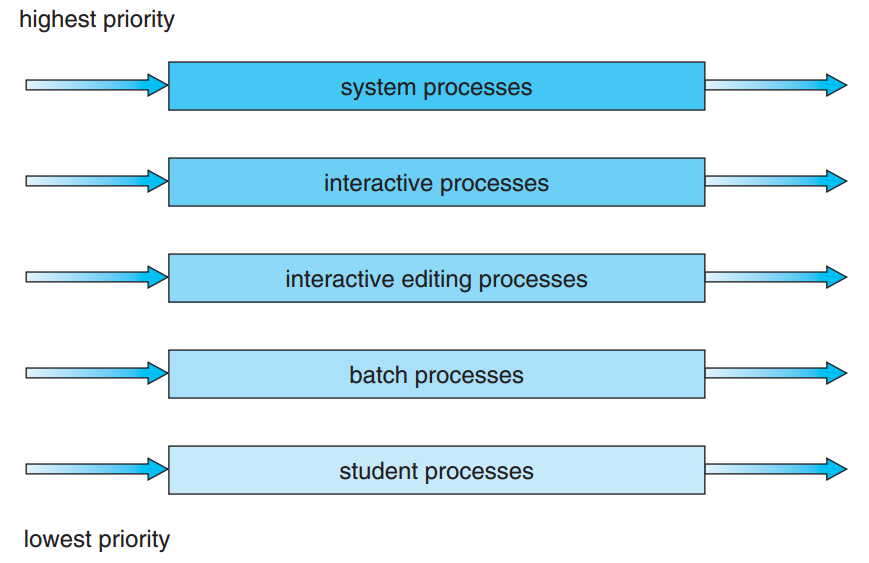
\includegraphics[width=0.6\textwidth]{img/mlq}
	\caption{\label{img:mlq}Colas y sus prioridades.}
\end{figure}
\newpage
%----------------------------------------------------------------------------------%


%--% Colas Multinivel con Retroalimentacion (MLFQ) %--------------------------------------%
{\centering \section{Colas Multinivel con Retroalimentacion (MLFQ)}}

Es parecido al MLQ, pero aqui los procesos no estan restringidos a quedarse en la cola en la que entraron,
pueden cambiar de una cola a otra.
Este algoritmo agrupa los procesos según las características de sus ráfagas de CPU, si un proceso
usa el CPU en mayor nivel, se pasa a una cola de prioridad mas baja. Esto deja a los procesos
limitados por E/S y los procesos interactivos en las colas con mayor prioridad.
Y los procesos que lleven mucho tiempo esperando en una cola de baja prioridad se pasa a una
cola de mayor prioridad (envejecimiento).

Para su implantación necesita el numero de colas, el algoritmo de planificación de cada cola,
el método usado para determinar cuando pasar un proceso a una cola de prioridad mas alta,
el método usado para determinar cuando pasar un proceso a una cola de prioridad mas baja
y el método usado para determinar en que cola se introducirá un proceso cuando haya que darle
servicio.

\begin{itemize}
	\item \textbf{Ventajas}
	\begin{itemize}
		\item Es general y adaptable a cualquier sistema.
	\end{itemize}
	
	\item \textbf{Desventajas}
	\begin{itemize}
		\item Es el algoritmo de planificacion mas complejo, requiere de algun mecanismo
		para definir el valor de todos los parametros.
	\end{itemize}
\end{itemize}

\vspace{0.1cm}
\begin{figure}[h]
	\centering
	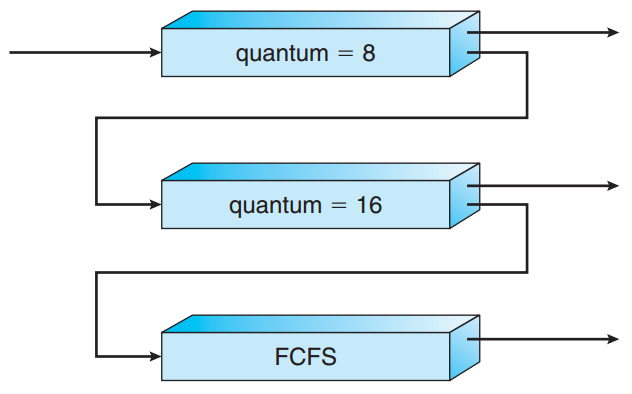
\includegraphics[width=0.6\textwidth]{img/mlfq}
	\caption{\label{img:mlq}Colas con diferentes algoritmos.}
\end{figure}

\newpage
%----------------------------------------------------------------------------------%


% Sistemas de Tiempo Real %--------------------------------------------------------%
\section*{Sistemas de Tiempo Real}
Es un sistema en el que se requiere no solo que los resultados calculados sean correctos,
sino que también se produzcan dentro de un periodo de tiempo especifico. Los procesos
deben terminar su ejecución en un periodo de tiempo. 

Esta los Soft Real-Time Systems, que no aseguran cuando un proceso sera ejecutado, pero garantiza que se la dará
preferencia (mas prioridad) sobre procesos no críticos.
Y los Hard Real-Time Systems, estos requieren que un proceso
termine su ejecución en un determinado tiempo, y si no
ocurre así el proceso es abortado.

Tenemos los siguientes métodos de planificación:

\begin{itemize}
	\item \textbf{Planificación de tablas estáticas}: Se conocen con anticipación los procesos a realizar, y se
	tratan como periódicos. Se planifican de tal modo que terminaran su ejecución antes del tiempo determinado
	incluso en las peores condiciones.
	
	\item \textbf{Planificación apropiativa con prioridad estática}: Se asignan prioridades a cada proceso relacionadas
	con el tiempo en que deban ser completados.
	
	\item \textbf{Planificación dinámica}: Se basa en realizar una prueba de factibilidad de manera dinámica (En tiempo de ejecución).
	Garantiza que un proceso terminara en el tiempo que debe realizando un plan de ejecución tomando en cuenta
	el tiempo que necesita para su peor caso y los recursos que necesita.
	
	\item \textbf{Dynamic best-effort}: Este es parecido a la planificación dinamica pero no realiza una prueba de factibilidad.
	El sistema hace lo que puede por cumplir los tiempos propuestos. Al no existir garantías, una tarea podría
	llegar a ser abortada durante su ejecución.
	
\end{itemize}
\newpage
%----------------------------------------------------------------------------------%


% Planificación para Linux %-------------------------------------------------------%
\section*{Planificación para Linux}

Linux provee soporte para sistemas SMP(Symmetric Multi-Processing o Multiprocesamiento Simétrico, 
es un tipo de arquitectura de computadores en la que dos o más unidades de procesamiento comparten 
una única memoria central.), y un algoritmo de planificacion que corre en tiempo \bigO{1} sin importar 
el numero de procesos. Linux asigna quantum de tiempo mas grande para procesos con mayor prioridad.
El algoritmo es basado en prioridades y apropiativo.
Linux asigna mas tiempo dedicado a las tareas de prioridad mas alta mas tiempo, y menos tiempo dedicado a las tareas
de prioridad mas baja.


\begin{figure}[h]
	\centering
	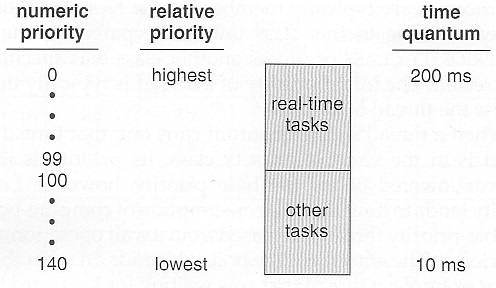
\includegraphics[width=0.5\textwidth]{img/5_15_PrioritiesVS_Length}
	\caption{\label{img:linux1}Relación entre prioridades y el tiempo dedicado que poseen.}
\end{figure}

El kernel mantiene una lista de todas las tareas ejecutables en una estructura de datos denominada cola de ejecución.
Debido al soporta para sistemas SMP, cada procesador mantiene su propia cola de ejecución y la planifica de forma
independiente. Cada cola de ejecución contiene dos matrices de prioridades, denominadas matrices activa y caducada.
Cada una de estas matrices de prioridades contiene una lista de tareas indexada en función de la prioridad.
Cuando todas las tareas han caducado sus tiempos totales (cuando la matriz activa está vacía), las dos matrices se intercambian.

\begin{figure}[h]
	\centering
	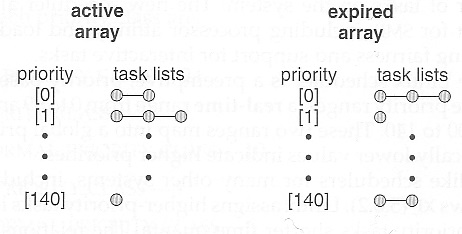
\includegraphics[width=0.5\textwidth]{img/5_16_TaskList}
	\caption{\label{img:linux2}Lista de tareas indexadas por prioridad.}
\end{figure}
\newpage
%----------------------------------------------------------------------------------%


%--% Planificación para Windows %--------------------------------------------------%
\section*{Planificación para Windows}

Windows usa un algoritmo apropiativo basado en prioridades.
El planificador se asegura que siempre se ejecute el hilo con la prioridad mas alta.
Existe un hilo especial ``Idle'' que se ejecuta cuando ningún otro hilo esta listo.
La parte del kernel de Windows que maneja la planificacion es llamada el despachador.

Existe una relación entre las prioridades del kernel de Windows y el API de Windows.
El API de Windows identifica 7 clases de prioridades (las filas de la tabla \ref{table:windows1})
y 6 prioridades relativas dentro de cada clase (las columnas de la tabla \ref{table:windows1}).
\begin{table}[h]
	\centering
	\begin{tabular}{l|l|l|l|l|l|l|}
		\cline{2-7}
		& Real-time & High & Above normal & Normal & Below normal & Idle priority \\ \hline
		\multicolumn{1}{|l|}{Time-critical} & 31        & 15   & 15           & 15     & 15           & 15            \\ \hline
		\multicolumn{1}{|l|}{Highest}       & 26        & 15   & 12           & 10     & 8            & 6             \\ \hline
		\multicolumn{1}{|l|}{Above normal}  & 25        & 14   & 11           & 9      & 7            & 5             \\ \hline
		\multicolumn{1}{|l|}{Normal}        & 24        & 13   & 10           & 8      & 6            & 4             \\ \hline
		\multicolumn{1}{|l|}{Below normal}  & 23        & 12   & 9            & 7      & 5            & 3             \\ \hline
		\multicolumn{1}{|l|}{Lowest}        & 22        & 11   & 8            & 6      & 4            & 2             \\ \hline
		\multicolumn{1}{|l|}{Idle}          & 16        & 1    & 1            & 1      & 1            & 1             \\ \hline
	\end{tabular}
		\caption{Clases de Prioridades de Windows}
		\label{table:windows1}
\end{table}

A cada proceso se le da una prioridad base dentro de su clase de prioridad. Cuando un proceso consume 
todo su tiempo disponible, su nivel de prioridad baja, pero nunca menos de su prioridad base.
A los procesos en primer plano se les multiplica su quantum de tiempo planificado (el tiempo total dedicado)
por 3, para que tengan mejor respuesta.
\newpage
%----------------------------------------------------------------------------------%


%--% Planificación en sistemas Multiprocesadores %--------------------------------------------------%
{\centering \section*{Planificación en sistemas Multiprocesadores}}

Cuando se tienen varios procesadores disponibles, la planificación se complica porque ahora
hay mas de un CPU al que se debe tener ocupado y en uso efectivo de manera constante.
Compartir la carga ayuda ya que balancea el trabajo entre múltiples procesadores.
Cuando se planifica para varios procesadores hay que tomar en cuenta si son distintos, o si son idénticos.

\begin{itemize}
	\item \textbf{Distintos (Sistema Heterogéneo)}: Cada procesador tiene su propia cola y algoritmo de
	planificación.
	
	\item \textbf{Idénticos (sistema homogéneo)}: Una solución podría ser el multiprocesamiento asimétrico, en el cual
	un procesador es el master (o líder), controla todas las actividades y corre todo el código
	del Kernel, mientras que los otros procesadores solo corren código de usuario. Esta solución es
	relativamente simple ya que no hay necesidad de compartir información critica del sistema.
	
	Por otro lado también esta el multiprocesamiento simétrico, en el cual cada procesador planifica sus
	propias tareas, ya sea de una cola en común o de colas separadas para cada procesador.
	Todos los sistemas operativos modernos soportan el multiprocesamiento simétrico.
\end{itemize}

%-------------------------------------------------------------------------------------------%


%--% Planificación en sistemas Multicore %--------------------------------------------------%
{\centering \section*{Planificación en sistemas Multicore}}

En el caso de sistemas Multicore, tenemos sistemas con múltiples procesadores pero en un solo
chip físico. A pesar de esta diferencia en hardware, el sistema operativo lo percibe de la misma manera,
como muchos procesadores a los que debe tener ocupado y en uso efectivo. Se ven mejoras en el consumo 
de energía.

\vspace{0.3cm}
%--------------------------------------------------------------------------------------------%


%--% Planificacion de hilos %--------------------------------------------------%
{\centering \section*{Planificacion de hilos}}
En el caso de los hilos, el sistema operativos planifica los hilos a nivel de kernel, los
hilos a nivel de usuario son gestionados por una librería de hilos y el kernel no es consciente
de ellos. Muchos sistemas consideran una estructura intermedia entre el hilo de kernel y el hilo
de usuario. Esta estructura es llamada Light Weight Process o LWP (proceso ligero) y es un medio para
lograr multitarea, se ejecuta en el espacio del usuario en la parte superior de un solo hilo de kernel,
es decir, por cada hilo de kernel le corresponde un LWP y este es el que planifica los hilos de usuario.

Para ejecutarse en el CPU los hilos de usuarios deben ser asignados a un hilo de nivel
de kernel asociado.

La biblioteca de hilos planifica los hilos de usuario para que se ejecuten sobre proceso LWP disponible,
lo cual es un esquema conocido con el nombre de ámbito de contienda del proceso(PCS, process contention scope),
dado que la competición por el CPU tiene lugar entre hilos que pertenecen al mismo proceso.
Para decidir que hilo del kernel planificar en un CPU, el kernel usa el ámbito de contienda del sistema (SCS),
la competición por el CPU con la planificacion SCS toma lugar entre todos los hilos del sistema.

\newpage
%----------------------------------------------------------------------------------%


%--% Criterios para evaluar los algoritmos %--------------------------------------------------%
{\centering \section*{Criterios para evaluar los algoritmos}}

El primer problema es definir el criterio utilizado para seleccionar un algoritmo.
El criterio es definido comúnmente por la utilización del CPU, tiempo de repuesta o el rendimiento.
Para seleccionar un algoritmo primero debemos definir la importancia de estos elementos.
Una vez definido el criterio a utilizar, podemos usar uno de los siguientes métodos:
\vspace{0.2cm}
\begin{itemize}
	\item \textbf{Modelado determinista}: es un tipo de evaluación analítica. Este método toma una carga de
	trabajo predeterminada y define el rendimiento de cada algoritmo para esa carga de trabajo. El modelado
	determinista es simple y rápido, nos da números exactos lo que nos permite comparar los algoritmos.
	\vspace{0.08cm}
	
	\item \textbf{Modelado de colas}: En muchos sistemas los procesos que son ejecutados varían de día a día, así
	que no existen un conjunto fijo de procesos para usar con modelado determinista. Sin embargo se puede determinar
	la distribución de las ráfagas de CPU y de E/S.
	El resultado es una formula matemática que describe la probabilidad de una ráfaga de CPU en particular.
	También se puede describir al distribución de los tiempos en que los procesos llegan al sistema.
	Con estas 2 distribuciones es posible calcular el rendimiento, utilización y tiempo de espera promedio
	para la mayoría de los algoritmos.
	
	El sistema informático se describe, dentro del modelado de colas, como una red de servidores. Cada servidor dispone
	de una cola de procesos en espera. El CPU es un servidor con su cola de procesos separados, al igual que el sistema
	de E/S con sus colas de dispositivos. Conociendo las tasas de llegada y el tiempo de servicio, podemos calcular la
	utilización, la longitud media ed las colas, el tiempo medio de espera, etc.
	
	La formula de Little (Little's Formula) dice que para una cola de longitud $n$, con un tiempo de espera promedio
	$W$ y una tasa media de llegada de nuevos procesos $\lambda$, la relación entre estos valores viene dada por:
	
	\begin{equation} \label{eq:little}
		n = \lambda \times W
	\end{equation}
	
	Podemos emplear esta formula para calcular una de las 3 variables si conocemos 2 de ellas.
	El análisis de colas puede resultar útil para comparar los distintos algoritmos de planificacion, aunque también
	tiene sus limitaciones. Por el momento, los algoritmos que pueden incluirse en el análisis son bastante limitados.
	Debido a esto y a otras dificultades, a menudo los modelos de cola sólo representan una aproximación a los sistemas 
	reales y la precisión de los resultados obtenidos puede ser cuestionable.
	\vspace{0.08cm}
	
	\item \textbf{Simulaciones}: Las simulaciones nos permiten obtener una evaluación mas precisa de los algoritmos
	de planificación. Ejecutar estas requiere programar un modelo del sistema informático. Los componentes
	principales del sistema se representan mediante estructuras de datos. El simulador tiene una variable que representa
	una señal del reloj, y cuando el valor de esta variable se incrementa, el simulador modifica el estado del sistema
	para reflejar las actividades de los dispositivos, los procesos y del planificador. A medida que se ejecuta
	la simulación las estadísticas que indican el rendimiento del algoritmo se recopilan y se envían a alguna salida.
	La información para ejecutar la simulación puede ser generada en diversas maneras, el método mas común usa un generador
	de números aleatorios que esta programado para generar procesos, tiempos de ráfaga de CPU, tiempos de llegada, tiempos de
	salida de acuerdo con una serie de distribuciones de probabilidad.
	
	Las simulaciones pueden ser costosas, en muchos casos requieren bastante tiempo de computo.
	Una simulación mas detallada provee resultados mas precisos, pero también requiere mas tiempo.
	\vspace{0.08cm}
	
	\item \textbf{Implementación}: La manera mas precisa de evaluar un algoritmo de planificacion, es programarlo
	y usarlo en un sistema operativo y observar como funciona. Este acercamiento nos permite observar
	el algoritmo bajo un sistema operativo en condiciones reales. La principal dificultad es su alto coste, que no solo viene
	de programar el algoritmo y modificar el sistema operativo para que lo soporte, sino también la reacción de los
	usuarios a un sistema operativo en constante cambio. La mayoría de los usuarios no están interesados en crear
	un sistema operativo mejor, simplemente quieren ejecutar sus procesos y utilizar los resultados obtenidos.
	
	Otra dificultad es que el entorno en el que se use el algoritmo esta sujeto a cambios. El entorno no cambiará
	unicamente de manera usual, a medida que se escriban nuevos programas y los tipos de problemas cambien, sino también
	como consecuencia del propio rendimiento del planificador.
	Si se da prioridad a los procesos cortos, entonces los usuarios pueden dividir los procesos largos en
	conjuntos de procesos mas cortos. Si se asigna una mayor prioridad a los procesos interactivos que a los no
	interactivos, entonces los usuarios pueden decidir utilizar procesos interactivos.
\end{itemize}


\newpage
%----------------------------------------------------------------------------------%

%%FIN CUERPO PRINCIPAl%%%%%%%%%%%%%%%%%%%%%%%%%%%%%%%%%%

%\newpage
%\section*{Glosario}
%\begin{itemize}
%	\item \textbf{Ráfaga CPU}: Tiempo de ejecución en CPU entre dos E/S.
%	\item \textbf{Ráfaga E/S}: Tiempo entre solicitud y terminación de E/S.
%\end{itemize}


% Bibliografia
%\cite{massachussetsUniversity, intef, jaume, Silberschatz, uic, presentacion, pag1}

\newpage

%--% Bibliografia %----------------------------------------------------------------%
\bibliographystyle{unsrt}
\bibliography{bibliography}
%----------------------------------------------------------------------------------%

\end{document}
